\documentclass[relatorio.tex]{subfiles}

\begin{document}
    
\subsection{Modelo do Sistema Solar} \label{subsec:sistema_solar}

O sistema solar foi atualizado, inserindo luzes e também as cores
e textura para cada modelo. Além disso também foi adicionado um 
cinturão de asteroides.

Como o sistema solar desenvolvido é apenas constituído por apenas uma estrela, que é
o sol, existe apenas uma única fonte de luz que é ponto situado no centro do sol (0, 0, 0). A 
luz trata-se de um ponto de maneira a emitir luz em todas as direções.

As texturas escolhidas para cada elemento do sistema foram retiradas do \textit{site Solar System Scope}.

As componentes da cor foram escolhidas de maneira a aproximar o modelo do sistema solar da realidade. 
\begin{itemize}
    \item A cor difusa para cada modelo foi escolhida com base na cor predominante da textura.
    \item A cor ambiente foi escolhida de forma a tentar representar a atmosfera envolvente.
    \item O único elemento que apresenta cor emissiva é o sol, uma vez que é o único que emite luz.
    \item Nenhum dos elementos do sistema solar verifica a reflexão especular logo a cor especular
    e a \textit{shininess} são sempre nulas.
\end{itemize}

Tal como referido anteriormente, foi adicionado o cinturão de asteroides que se situa entre Marte e 
Júpiter. O cinturão possui um movimento de rotação sobre o sol.

\begin{landscape}
    \begin{figure}
        \centering
        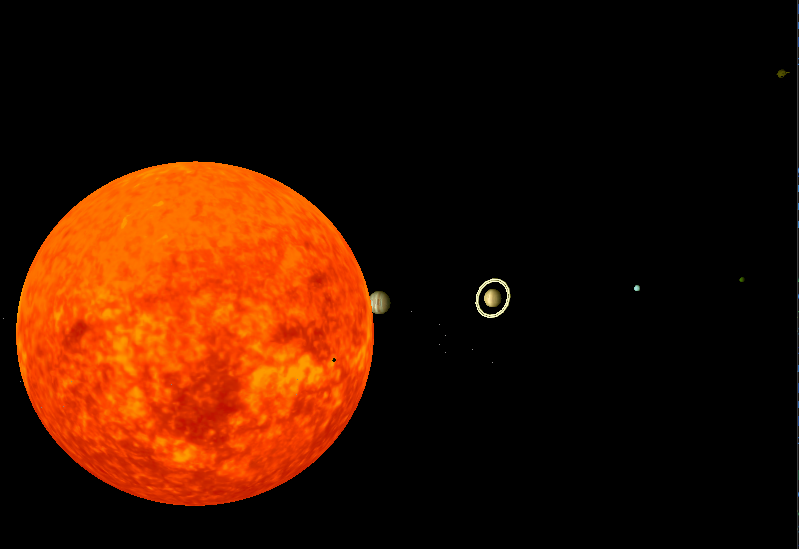
\includegraphics[width=\linewidth]{assets/sis_solar1.png}
        \caption{Sistema solar 1} \label{fig:sistema_solar_1}
    \end{figure}
\end{landscape}

\begin{landscape}
    \begin{figure}
        \centering
        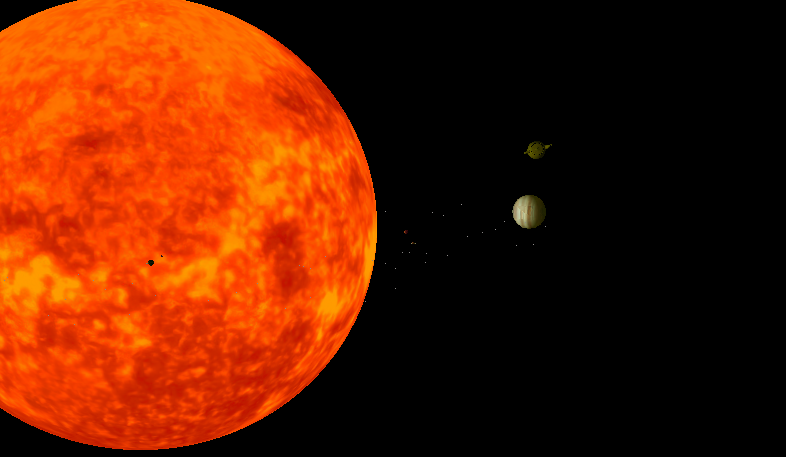
\includegraphics[width=\linewidth]{assets/sis_solar2.png}
        \caption{Sistema solar 2} \label{fig:sistema_solar_2}
    \end{figure}
\end{landscape}

\end{document}